\documentclass[12pt]{article}
\usepackage[margin=1.2in]{geometry}
%\usepackage{physics}
\usepackage{graphicx}
\usepackage{newpxtext,newpxmath}
%\usepackage{caption}
\usepackage{amsmath}
\usepackage[shortlabels]{enumitem}
\usepackage{amssymb}
%\usepackage{bm}
\usepackage{framed}
%\usepackage{authblk}
\usepackage{hyperref}
\usepackage{xcolor}
\hypersetup{
	colorlinks,
	linkcolor={black!50!black},
	citecolor={blue!50!black},
	urlcolor={blue!80!black}
}
\usepackage{MnSymbol,wasysym}
%\usepackage{empheq}
\usepackage{amsfonts}
%\usepackage{esint}
%\usepackage[makeroom]{cancel}
%\usepackage{dsfont}
%\usepackage{centernot}
%\usepackage{mathtools}
%\usepackage{bigints}
%\usepackage{amsthm}
%\theoremstyle{definition}
%\newtheorem{defn}{Definition}[section]
%\newtheorem{prop}{Proposition}[section]
%\newtheorem{rmk}{Remark}[section]
%\newtheorem{thm}{Theorem}[section]
%\newtheorem{exmp}{Example}[section]
%\newtheorem{prob}{Problem}[section]
%\newtheorem{sln}{Solution}[section]
%\newtheorem*{prob*}{Problem}
%\newtheorem{exer}{Exercise}[section]
%\newtheorem*{exer*}{Exercise}
%\newtheorem*{sln*}{Solution}
%\usepackage{empheq}
%\usepackage{hyperref}
%\usepackage{tensor}
%\usepackage{xcolor}
%\hypersetup{
%	colorlinks,
%	linkcolor={black!50!black},
%	citecolor={blue!50!black},
%	urlcolor={blue!80!black}
%}





%\newcommand*\widefbox[1]{\fbox{\hspace{2em}#1\hspace{2em}}}

\newcommand{\p}{\partial}
\newcommand{\R}{\mathbb{R}}
\newcommand{\C}{\mathbb{C}}
\newcommand{\lag}{\mathcal{L}}
\newcommand{\nn}{\nonumber}
\newcommand{\ham}{\mathcal{H}}
\newcommand{\M}{\mathcal{M}}
\newcommand{\I}{\mathcal{I}}
\newcommand{\K}{\mathcal{K}}
\newcommand{\F}{\mathcal{F}}
\newcommand{\w}{\omega}
\newcommand{\lam}{\lambda}
\newcommand{\al}{\alpha}
\newcommand{\be}{\beta}
\newcommand{\x}{\xi}

\newcommand{\G}{\mathcal{G}}

\newcommand{\f}[2]{\frac{#1}{#2}}

\newcommand{\ift}{\infty}

\newcommand{\lp}{\left(}
\newcommand{\rp}{\right)}

\newcommand{\lb}{\left[}
\newcommand{\rb}{\right]}

\newcommand{\lc}{\left\{}
\newcommand{\rc}{\right\}}


\newcommand{\V}{\mathbf{V}}
\newcommand{\U}{\mathcal{U}}
\newcommand{\Id}{\mathcal{I}}
\newcommand{\D}{\mathcal{D}}
\newcommand{\Z}{\mathcal{Z}}

%\setcounter{chapter}{-1}


%\makeatletter
%\renewcommand{\@chapapp}{Part}
%\renewcommand\thechapter{$\bf{\ket{\arabic{chapter}}}$}
%\renewcommand\thesection{$\bf{\ket{\arabic{section}}}$}
%\renewcommand\thesubsection{$\bf{\ket{\arabic{subsection}}}$}
%\renewcommand\thesubsubsection{$\bf{\ket{\arabic{subsubsection}}}$}
%\makeatother



\usepackage{subfig}
\usepackage{listings}
\captionsetup[lstlisting]{margin=0cm,format=hang,font=small,format=plain,labelfont={bf,up},textfont={it}}
\renewcommand*{\lstlistingname}{Code \textcolor{violet}{\textsl{Mathematica}}}
\definecolor{gris245}{RGB}{245,245,245}
\definecolor{olive}{RGB}{50,140,50}
\definecolor{brun}{RGB}{175,100,80}
\lstset{
	tabsize=4,
	frame=single,
	language=mathematica,
	basicstyle=\scriptsize\ttfamily,
	keywordstyle=\color{black},
	backgroundcolor=\color{gris245},
	commentstyle=\color{gray},
	showstringspaces=false,
	emph={
		r1,
		r2,
		epsilon,epsilon_,
		Newton,Newton_
	},emphstyle={\color{olive}},
	emph={[2]
		L,
		CouleurCourbe,
		PotentielEffectif,
		IdCourbe,
		Courbe
	},emphstyle={[2]\color{blue}},
	emph={[3]r,r_,n,n_},emphstyle={[3]\color{magenta}}
}






\begin{document}

\begin{center}
	\LARGE{\textbf{MIDTERM}}
	\\
	\large{Huan Q. Bui}
	
	\noindent \hrulefill\\
	\small{MA434: Algebraic Geometry}\\
	\small{March 9-13, 2020}\\\vspace{-6pt}
	\hrulefill
\end{center}


$\,$\\
$\,$\\


\begin{center}
\begin{tabular}{|c|c|c|}
	\hline
	Problem & Earned & Total\\
	\hline
	1&&20\\
	\hline
	2&&20\\
	\hline
	5&&20\\
	\hline
	6&&20\\
	\hline
	8&&20\\
	\hline
	10&&20\\
	\hline
	11&&20\\
	\hline
	\textbf{Total}&$\,\quad\quad$/100&120\\
	\hline
\end{tabular}
\end{center}



\newpage




\section*{Problem 1 \small{(20 pts)}}
Suppose $f(X,Y,Z)$ is a homogeneous polynomial of degree $n$ with coefficients in $\mathbb{R}$, so that we have $f(tX,tY,tZ) = t^n(X,Y,Z)$. Show that
\begin{align*}
X\f{\p f}{\p X} + Y\f{\p f}{\p Y} + Y\f{\p f}{\p y}  = nf.
\end{align*}
(Hint: this is true for any differentiable function that satisfies the equation $f(tX,tY,tZ) = t^n f(X,Y,Z)$, not just for polynomials; use calculus.)\\

It's worth point out that this shows that if a point $P$ satisfies 
\begin{align}\label{eq2}
\f{\p f}{\p X}\bigg\vert_P = \f{\p f}{\p X}\bigg\vert_P  = \f{\p f}{\p X}\bigg\vert_P = 0,
\end{align}
then $P$ is automatically on the curve defined by $f(X,Y,Z) = 0$.\\











\noindent \textbf{Solution:} Let such a function $f$ be given. Since $f$ is a polynomial in $X,Y,Z$, it is an everywhere-differentiable function. This allows us to use calculus without ``worries.'' Consider the change of variables $(X,Y,Z) \xrightarrow{t} (X',Y',Z')$ given by $X'=tX; Y'=tY, Z'=tZ$. We look at the following chain of implications
\begin{align*}
f(X',Y',Z') &= t^n f(X,Y,Z), \quad \text{(hypothesis)}\nn\\
\f{\p}{\p t} f(X',Y',Z') &= \f{\p }{\p t} [t^n f(X,Y,Z)]\nn\\
\f{\p X'}{\p t}\f{\p f}{\p X'} + \f{\p Y'}{\p t}\f{\p f}{\p Y'} + \f{\p Z'}{\p t}\f{\p f}{\p Z'} &= nt^{n-1}f(X,Y,Z), \quad \text{(chain rule)}\nn\\
X\f{\p f}{\p X'} + Y\f{\p f}{\p Y'} + Z\f{\p f}{\p Z'}&= nt^{n-1}f(X,Y,Z)
\end{align*}
This last equality holds for all $t$. Setting $t=1$, we have $X' = tX = X, Y'=Y, Z'=Z$, and thus it follows that
\begin{align*}
X\f{\p f}{\p X} + Y\f{\p f}{\p Y} + Z\f{\p f}{\p Z}= nf(X,Y,Z).
\end{align*}
For any point $P = (\bar{X},\bar{Y}, \bar{Z})$ such that Eq. \eqref{eq2} is satisfied, $nf(P) = 0$ automatically and thus $f(P) = 0$, i.e., $P$ is on the curve defined by $f(X,Y,Z) = 0$. 

\hfill $\square$

\newpage



\section*{Problem 2 \small{(20 pts)}}
The Proposition in section 1.13 of \textit{Undergraduate Algebraic Geometry} says that in a pencil of conics \textit{containing at least one non-degenerated conic} there will be at most 3 degenerate conics, and if $k = \mathbb{R}$ there will always be at least one degenerate conic. Find an example of a pencil of conics over $\mathbb{R}$ that does not contain any non-degenerate conics. \\





\noindent \textbf{Solution:} Call $C_{(\lambda,\mu)}: (\lambda Q_1 + \mu Q_2 = 0)$ the desired pencil of conics. The Proposition in 1.13 of Reid's says that if $C_{(\lambda,\mu)}$ contains at least one non-degenerate conic and if $k=\mathbb{R}$, then $C_{(\lambda,\mu)}$ contains \textit{at least one} degenerate conic. This means we want our desired $C_{(\lambda,\mu)}$ to be degenerate.\\

\noindent The condition that $C_{(\lambda,\mu)}$ contains at least one non-degenerate conic is equivalent to $F_{(\lambda,\mu)}$ not identically zero where
$F_{(\lambda,\mu)} = \det(\lambda Q_1 + \mu Q_2)$,
with $Q_1, Q_2$ written as $3\times 3$ symmetric matrices. So, our $C_{(\lambda,\mu)}$ must be such that $F_{(\lambda,\mu)}$ is identically zero. In fact, $C_{(\lambda,\mu)} \text{ degenerate} \iff F_{(\lambda,\mu)} = \det(\lambda Q_1 + \mu Q_2) = 0\, \forall \, \lambda,\mu \in \mathbb{R}$.\\

\noindent \underline{Goal}: to find $Q_1, Q_2$ such that $F_{(\lambda,\mu)}$ is identically zero, i.e.,
\begin{align*}
\det \lb \lambda \underbrace{\begin{pmatrix}
a&b&d\\b&c&e\\d&e&f
\end{pmatrix}}_{Q_1} 
+
\mu \underbrace{\begin{pmatrix}
a'&b'&d'\\b'&c'&e'\\d'&e'&f'
\end{pmatrix}}_{Q_2}\rb \equiv 0.
\end{align*}
where 
\begin{align*}
Q = aX^2 + 2bXY + cY^2 + 2dXZ + 2eYZ + fZ^2 \longleftrightarrow \begin{pmatrix}
a&b&d\\b&c&e\\d&e&f
\end{pmatrix}.
\end{align*}
Consider $Q_1 = -X^2 + Y^2$ and $Q_2 = 2XY + 2YZ$, then 
\begin{align*}
F_{(\lambda,\mu)} = \det 
\lb 
\lambda \underbrace{\begin{pmatrix}
-1&&\\&1&\\&&0
\end{pmatrix}}_{Q_1} 
+
\mu \underbrace{\begin{pmatrix}
&1&\\1&&1\\&1&
\end{pmatrix}}_{Q_2} 
\rb 
= \det \begin{pmatrix}
-\lambda & \mu & 0 \\\mu & \lambda & \mu \\ 0 & \mu & 0
\end{pmatrix} = \lambda \mu^2 - \mu^2 \lambda = 0.
\end{align*}
This holds for all $\lambda,\mu$. So, $C_{(\lambda,\mu)}$ generated by the conics $C_1:(Q_1 = -X^2 + Y^2=0)$ and $C_2: (Q_2 = 2XY + 2YZ =0) $ is degenerate $\iff$ $C_{(\lambda,\mu)}$ contains no non-degenerate conics. Not surprisingly, both $C_1$ and $C_2$ look like lines. 

\hfill$\square$




\newpage


\section*{Problem 5 \small{(20 pts)}} 


This problem describes another way of thinking about the projective line $\mathbb{P}^1(k)$. Remember that the affine line $\mathbb{A}^1(k)$ is just another name for the field $k$. \\

Any point in $\mathbb{P}^1(k)$ looks like $[u:v]$ with $u,v \in k$. Define the subsets
\begin{align*}
U = \lc [u:v]\in \mathbb{P}^1(k) \,\vert\, v \neq 0  \rc
\end{align*}
and
\begin{align*}
V = \lc [u:v]\in \mathbb{P}^1(k) \,\vert\, u \neq 0  \rc.
\end{align*}
\begin{enumerate}[(a)]
	\item If $[u:v] \in U$, define $f([u:v]) = u/v$. Show that $f$ is a bijection between $U$ and $\mathbb{A}^1(k)$. 
	\item If $[u:v] \in U$, define $g([u:v]) = v/u$. Show that $g$ is a bijection between $V$ and $\mathbb{A}^1(k)$. 
	\item Suppose $t \in \mathbb{A}^1(k), t\neq 0$, What is $f(g^{-1}(t))$?
	\item Explain how this means that we can think of $\mathbb{P}^1(k)$ as the result of gluing two copies of $\mathbb{A}^1(k)$ along the subsets $A^1(k)\setminus \{0\}$ via the function $t \to 1/t$. (If you prefer to avoid the language of ``gluing,'' you can express it as taking the disjoint union of two copies of $A^1(k)$ and then passing to the quotient with respect to an equivalence relation.) 
\end{enumerate}



\noindent \textbf{Solution:} 


\begin{enumerate}[(a)]
	\item 
	\item 
	\item 
	\item 
\end{enumerate}





\newpage

















\section*{Problem 6 \small{(20 pts)}}

Let $E$ be the cubic in $\mathbb{P}^2(\mathbb{Q})$ defined by the affine equation in Weierstrass form
\begin{align*}
y^2 = x^3 + x + 1.
\end{align*}
The point $P = (0,1)$ is on $E$. Use the group law to compute $2P$, $3P$, and $4P$. (The numbers will get ugly, so use software. It's ok to use \textit{Sage}'s built-in functions if you can figure out how to do it.)\\





\noindent \textbf{Solution:} \\

\noindent $\boxed{2P}$ To find $2P$, we want to find the inverse of the third intersection of the tangent line to $E$ through $P=(0,1)$. Let $f(x,y) = y^2 - x^3 - x - 1$. This tangent line is given by
\begin{align*}
\f{\p f}{\p x}(P)(x-0) + \f{\p f}{\p y}(P)(y-1) &= 0\nn\\
(-3\cdot 0^2-1)x + 2(y-1) &= 0 \implies {y = \f{1}{2}x + 1}
\end{align*}
The third intersection (since $P$ is a double intersection) of the tangent line and $E$:
\begin{align*}
\lp \f{1}{2}x + 1 \rp^2 = x^3 + x + 1, \quad \text{with }x\neq 0 \iff  x = \f{1}{4} \implies y = \f{1}{2}\cdot\f{1}{4} + 1 = \f{9}{8}.
\end{align*}
$2P$ is the inverse of this point (obtained by flipping the sign of the $y$-coordinate):
\begin{align*}
\boxed{2P = \lp \f{1}{4}, \f{-9}{8} \rp}
\end{align*}
\textit{Mathematica code:}
\begin{lstlisting}
Solve[((1/2) x + 1)^2 == x^3 + x + 1, x]
{{x -> 0}, {x -> 0}, {x -> 1/4}}
\end{lstlisting}
$\,$\\
\noindent $\boxed{3P}$ We repeat this process for $3P$. The line through $P$ and $2P$ is given by
\begin{align*}
y = -\f{17}{2}x + 1.
\end{align*}
We rely on Mathematica to find the third intersection of this line with $E$. Taking the inverse of this third point, we get $3P$:
\begin{align*}
\boxed{3P =  \lp 72, +611 \rp}
\end{align*}
\noindent \textit{Mathematic code:}
\begin{lstlisting}
Solve[(-(17/2) x + 1)^2 == x^3 + x + 1, x]
{{x -> 0}, {x -> 1/4}, {x -> 72}}

-(17/2) 72 + 1
-611
\end{lstlisting}
$\,$\\
\noindent $\boxed{4P}$ We do this once again to find $4P$. The line through $3P$ and $P$ is given by
\begin{align*}
y =  \f{610}{72}x + 1.
\end{align*}
(where I'm leaving the fraction unsimplified to make checking easier). Using Mathematica, we find the third intersection of this line with $E$. Taking the inverse of this third point, we get $4P$:
\begin{align}
\boxed{ 4P =\lp \f{-287}{1296}, \f{40879}{46656} \rp }
\end{align}


\textit{Mathematica code:}
\begin{lstlisting}
Solve[((610/72) x + 1)^2 == x^3 + x + 1, x]
{{x -> -(287/1296)}, {x -> 0}, {x -> 72}}

(610/72) (-(287/1296)) + 1
-(40879/46656)
\end{lstlisting}


$\,$\\

\noindent $\boxed{4P, \text{ bis}}$ As a check, we can find $4P$ via $2P + 2P$ as well. In this case, we consider the line through $2P$ tangent to $E$. This line is given by
\begin{align}
\lp -3 \cdot \lb \f{1}{4} \rb^2 - 1 \rp \lp x - \f{1}{4} \rp + 2\lp\f{-9}{8}\rp\lp y + \f{9}{8} \rp = 0 \implies y = -\f{19}{36}x - \f{143}{144}.
\end{align}
We find the third intersection of this line and $E$ and invert it to get the same $4P$, as expected. \\

\noindent \textit{Mathematica code:}
\begin{lstlisting}
Solve[(-(143/144) - (19 x)/36)^2 == x^3 + x + 1, x]
{{x -> -(287/1296)}, {x -> 1/4}, {x -> 1/4}}

-(143/144) - (19 (-(287/1296)))/36
-(40879/46656)
\end{lstlisting}  







































\newpage


\section*{Problem 8 \small{(20 pts)}}
(Gauss's Lemma) Suppose $R$ is a UFD and $K$ is its field of fractions. We want to compare factorizations in $R[x]$ and in $K[x]$. Let $f(x)\in R[x]$ and suppose we have $g(x), h(x) \in K[x]$ such that $f(x) = g(x)h(x)$. Show that there exists $a\in K$ such that $\tilde g(x)=  ag(x) \in R[x]$, and $\tilde h(x) = \f{1}{a}h(x) \in R[x]$, and so $f(x) = \tilde g(x) \tilde h(x)$ is a factorization in $R[x]$. (It's useful to remember that in a UFD every irreducible element is prime and that if $D$ is a domain so is $D[x]$.) \\



\noindent \textbf{Solution:} (\textit{inspired by the proofs of Gauss's Lemma \& reducibility over $\mathbb{Q}[x] \implies$ reducibility over $\mathbb{Z}[x]$ by Gallian}) Let any $f(x) \in R[x]$ be given. We can factor out the content $c \in R$ of $f(x)$ so that $f(x) = cf_1(x)$ where $f_1$ is \textit{primitive} (i.e., the coefficients of $f_1(x)$ have no irreducible factors in common). We first want to show that the product of two primitive polynomials is primitive. 

\begin{framed}
\noindent \underline{To prove}: The product of two primitive polynomials is primitive.\\

Let $\mathfrak{f}(x),\mathfrak{g}(x) \in R[x]$ be primitive polynomials. Suppose (to get a contradiction) that $\mathfrak{f}(x)\mathfrak{g}(x)$ is not primitive. Let $p$ be an irreducible element of $R$ (hence prime because $R$ is a UFD) such that $p$ divides the ``gcd'' of the coefficients of $\mathfrak{f}(x) \mathfrak{g}(x)$. Let $\bar{\mathfrak{f}}(x)$, $\bar{\mathfrak{g}}(x)$, and $\overline{\mathfrak{f}(x)\mathfrak{g}(x)}$ be the polynomials obtained from $\mathfrak{f}(x)$, $\mathfrak{g}(x)$, and $\mathfrak{f}(x)\mathfrak{g}(x)$ by reducing the coefficients ``mod'' $p$. \\

We consider the function $\phi: R[x] \to R_p[x]$ defined by 
\begin{align*}
\phi \lp \sum^n_{i=1}a_i x^i \rp = \sum^n_{i=1}\bar{a}_ix^i
\end{align*}
where $\bar{a} = a\mod p$. This is a ring homomorphism:
\begin{itemize}
	\item $\phi(\mathfrak{f} + \mathfrak{g}) = \phi(\mathfrak{f}+\mathfrak{g})$:
	\begin{align*}
	\phi\lp \sum^n_{i=1}a_i x^i + \sum^m_{i=1}b_i x^i \rp = \sum^n_{i=1}\bar{a}_i x^i + \sum^m_{i=1}\bar{b}_i x^i = \phi\lp \sum^n_{i=1}a_i x^i \rp + \phi\lp \sum^m_{i=1}b_i x^i \rp.
	\end{align*}
	\item $\phi(\mathfrak{f}\mathfrak{g}) = \phi(\mathfrak{f})\phi(\mathfrak{g})$:
	\begin{align*}
	\phi\lp \sum^n_{i=1}a_i x^i \cdot \sum^m_{i=1}b_i x^i \rp= \sum_{i=1}^n\sum^m_{j=1}\bar{a}_i\bar{b}_j x^{i+j} = \phi\lp \sum^n_{i=1}a_i x^i \rp \phi\lp \sum^m_{i=1}b_i x^i \rp.
	\end{align*}
\end{itemize}





So, $\bar{\mathfrak{f}}(x)$ and $\bar{\mathfrak{g}}(x)$ belong to $R_p[x]$, which we can see is an integral domain. Further, because the coefficients of $\mathfrak{f}(x)\mathfrak{g}(x)$ have $p$ as a common factor (assumption), $\bar{\mathfrak{f}}(x)\bar{\mathfrak{g}}(x) = \overline{\mathfrak{f}(x)\mathfrak{g}(x)} = 0$, the zero element of $R_p[x]$. Therefore, $\bar{\mathfrak{f}}(x) = 0$ or $\bar{\mathfrak{g}}(x) = 0$, and so $p$ divides every coefficient of $\mathfrak{f}(x)$ or $p$ divides every coefficient of $\mathfrak{g}(x)$. This implies that either $\mathfrak{f}(x)$ is not primitive or $\mathfrak{g}(x)$ is not primitive. This contradicts our initial assumption. So $\mathfrak{f}(x)\mathfrak{g}(x)$ must be primitive. \hfill$\triangle$
\end{framed}


Back to our proof. Suppose we have $g(x),h(x) \in K[x]$ such that 
\begin{align*}
f_1(x) = g(x)h(x) \in R[x]
\end{align*}
(remember that $f_1(x)$ is the primitive polynomial constructed from $f(x)$). Let $\gamma$ be the ``lcm'' of the denominators of the coefficients of $g(x)$, and $\eta$ the ``lcm'' of the denominators of the coefficients of $h(x)$. Then we have $\gamma\eta f_1(x) = \gamma g(x) \cdot \eta h(x)$, where $\gamma g(x), \eta h(x) \in R[x]$. Let $c_1$ be the content of $\gamma g(x)$ and $c_2$ the content of $\eta h(x)$. Then,
\begin{align*}
&\gamma g(x) = c_1 \tilde{g}(x)\nn\\
&\eta h(x) = c_2 \tilde{h}(x)\nn
\end{align*}  
where both $\tilde{g},\tilde{h}$ are primitive polynomials in $R[x]$. With this, we have
\begin{align}\label{eq3}
\gamma \eta f_1(x) = c_1 c_2 \tilde{g}(x)\tilde{h}(x).
\end{align}
Now, $f_1(x)$ is primitive, so the content of $\gamma \eta f_1(x)$ is $\gamma \eta$. $\tilde{g}(x)\tilde{h}(x)$ is primitive (because $\tilde{g}(x),\tilde{h}(x)$ are primitive), so the content of $\gamma \eta \tilde{g}(x)\tilde{h}(x)$ is $\gamma\eta$. From here, we see that $\gamma \eta = c_1 c_2$, and thus $f_1(x) = \tilde{g}(x)\tilde{h}(x) \in R[x]$.  In particular, because $\gamma \eta = c_1 c_2$, we can call
\begin{align*}
a = \f{\gamma}{c_1} = \f{c_2}{\eta} \in K,
\end{align*}
so that we can write, from \eqref{eq3},
\begin{align*}
f_1(x) = \tilde{g}(x)\tilde{h}(x) =  \f{\gamma}{c_1} \tilde{g}(x) \f{c_2}{\eta}\tilde{h}(x) = a g(x) \f{1}{a}h(x).
\end{align*}
Obviously, 
\begin{align*}
ag(x) &= \f{\gamma}{c_1}g(x) = \tilde{g}(x) \in R[x]\nn\\
\f{1}{a}h(x) &= \f{\eta}{c_2}h(x) = \tilde{h}(x) \in R[x].
\end{align*}
So, we have shown that there exists $a \in K$ such that $\tilde{g}(x) = ag(x) \in R[x]$, $\tilde{h}(x) = \f{1}{a}h(x) \in R[x]$, and thus $f_1(x) = \tilde{g}(x)\tilde{h}(x)$ is a factorization in $R[x]$. To recover $f(x)$ from $f_1(x)$ we can just let $\tilde{g}(x)$ absorb the content $c$ of $f(x)$. Because $\tilde{g} \to c\tilde{g}$ must still be in $R[x]$, we get the factorization $f(x) = \tilde{g}(x)\tilde{h}(x)$ in $R[x]$.   

\hfill$\square$ 




















\newpage


\section*{Problem 10 \small{(20 pts)}}

Let $C$ be the curve in $\mathbb{P}^2$ whose affine equation is $y^2 = x^3 + x^2$. This is the modal cubic we studied in section 2.1. Show that the line $y=tx$ has a double intersection with $C$ at $(0,0)$ and find the third point of intersection. Check that this gives the parameterization in 2.1. What happens when $t = \pm 1$? \\



\noindent \textbf{Solution:} The $x-$coordinate of any intersection between the line $y = tx$ and the nodal cubic $y^2 = x^3 + x^2$ satisfies the equation:
\begin{align*}
(tx)^2 = x^3 + x^2 &\iff x^3 + (1-t^2)x^2 = 0 \nn\\
&\iff x^2(x + 1 -t^2) = 0.
\end{align*}
Clearly, there is a double root at $x=0$. Thus, the point $(x,tx) = (0,0)$ is a double intersection. \\

\noindent The $x-$coordinate of the third point of intersection solves the equation $x + 1 - t^2 = 0 \iff x = t^2 - 1$. Plugging this into the equation for the line, we get the third point of intersection:
\begin{align}
(x,y) = (t^2 - 1, t^3 - t).
\end{align}
This is exactly the parameterization in 2.1. of Reid's.\\

\noindent When $t = \pm 1$, the third point of intersection is once again $(0,0)$, making $(0,0)$ a triple intersection. Both the lines $y = x$ and $y = -x$ are tangents to $E$ at $(0,0)$. Intuitively, we can think about the triple intersection as three intersections, one of which due to one ``branch'' of the cubic and the other two is a double root on the other ``branch.'' If we associate each line $y = \pm x$ to the correct ``branch'' of the cubic, we see that they are both tangent lines. \\

\noindent To see this more explicitly, we can consider the ``branch'' given by the parameterization:
\begin{align}
t \to \begin{cases}
(t, \sqrt{t^3+t^2}), &\quad t \geq 0\\
(t, -\sqrt{t^3+t^2}), &\quad t < 0
\end{cases}
\end{align} 
The line $y = x$ is tangent to this branch of $C$ at $(0,0)$. We can see that
\begin{align}
\lim\limits_{h \downarrow 0} \f{\sqrt{h^3+h^2} - 0}{h} =  1 = \lim\limits_{h\uparrow 0}\f{-\sqrt{h^3+h^2} - 0}{h},
\end{align}
which implies the slope of this branch at $(0,0)$ is 1, and so we see that $y=x$ is tangent to $C$ here. Following a similar argument, we can see that $y = -x$ is tangent to the other branch of this cubic, again at $(0,0)$. 


\newpage

\begin{figure}[!htb]
	\centering
	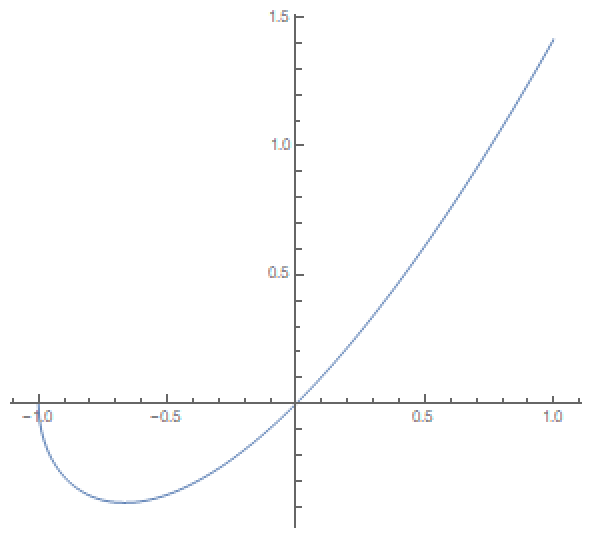
\includegraphics[scale=0.7]{ag1}
	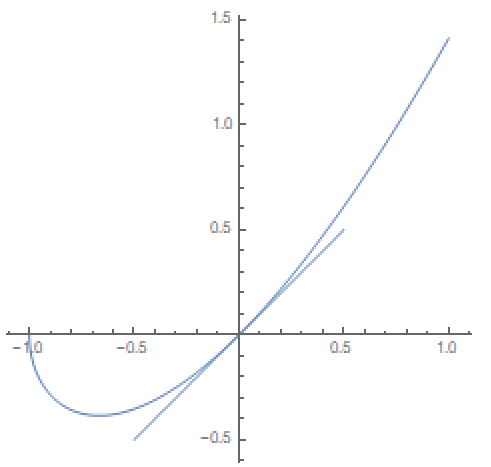
\includegraphics[scale=0.7]{ag2}
	\caption{A ``branch'' of the nodal cubic and the tangent line $y=x$}
\end{figure}
\begin{figure}[!htb]
	\centering
	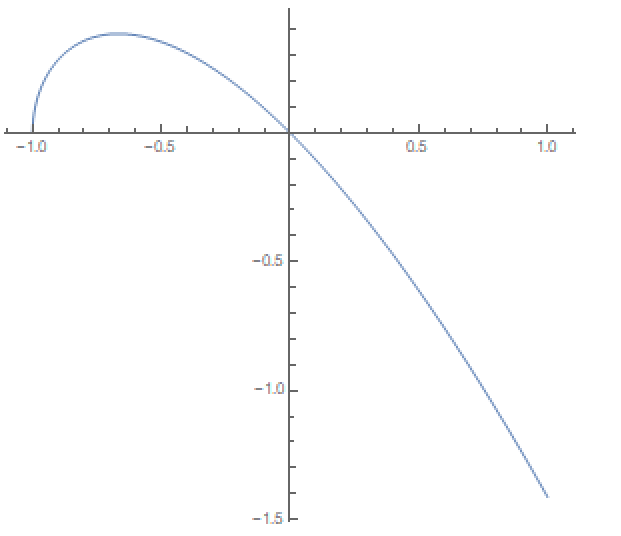
\includegraphics[scale=0.7]{ag3}
	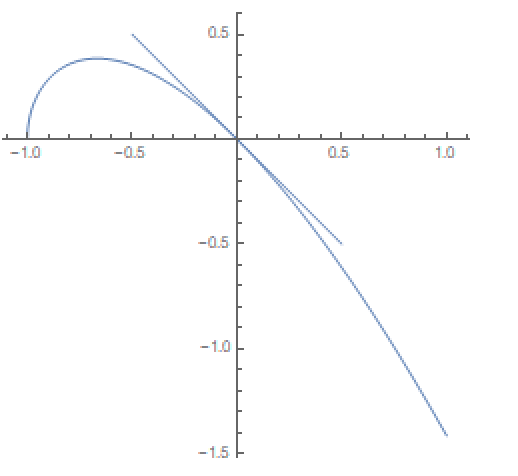
\includegraphics[scale=0.7]{ag4}
	\caption{Another ``branch'' of the nodal cubic and the tangent line $y=-x$}
\end{figure}
Putting these pictures together we get two distinct tangents at $(0,0)$:
\begin{figure}[!htb]
	\centering
	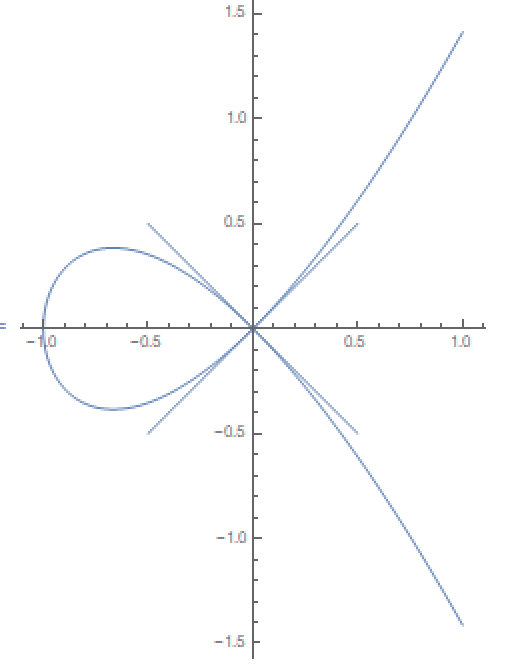
\includegraphics[scale=0.6]{ag5}
	\caption{Another ``branch'' of the nodal cubic and the tangent line $y=-x$}
\end{figure}



\hfill $\square$


\newpage


\section*{Problem 11 \small{(20 pts)}}

With $C$ as in the previous problem, let $C(k)$ be the set of points on $C$ with coefficients in $k$ (including the point at infinity), and let $C'(k) = C(k)\setminus \{(0,0)\}$. (S $C'(k)$ is the set of points on $C$ where there is a unique tangent.) We want to try to define a group structure using the same method as for nonsingular cubics. 
\begin{enumerate}[(a)]
	\item Let $A$ be a point in $C(k)$ and let $P = (0,0)$. Let $L$ be the line through $A$ and $P$. What is the third intersection of $L$ and $C$?
	\item Explain why the point $P$ is problematic if we want a group structure.
	\item Suppose $A,B \in C'(k)$, and let $L$ be the line through $A$ and $B$. Show that the third intersection of $L$ with $C$ is in $C'(k)$. 
	\item Explain why this gives a group law on $C'(k)$. 
\end{enumerate}

\noindent (It turns out that this group law $C'(k) \cong k^\times$, but this is a little hard to prove. )\\



\noindent \textbf{Solution:}

\begin{enumerate}[(a)]
	\item 
	\item 
	\item 
	\item 
\end{enumerate}


\newpage



\section*{Acknowledgments/References}

I've referred to...




	
\end{document}